\documentclass[xetex,mathserif,serif,aspectratio=169]{beamer}

\usepackage{xltxtra}
\usepackage{color}
\usepackage{url}
\usepackage{listings}
\usepackage{fontspec}
\usepackage{geometry}
\usepackage{lastpage}
\usepackage{fancyhdr}
\usepackage{amsmath}
\usepackage{amsthm}
\usepackage{amssymb}
\usepackage{blkarray}
\usepackage{multicol}
\usepackage{relsize}
\usepackage{listings}
\usepackage{xunicode}
\usepackage{xltxtra}
\usepackage{color}
\usepackage{url}
\usefonttheme[onlymath]{serif}

\definecolor{solarized@base03}{HTML}{002B36}
\definecolor{solarized@base02}{HTML}{073642}
\definecolor{solarized@base01}{HTML}{586e75}
\definecolor{solarized@base00}{HTML}{657b83}
\definecolor{solarized@base0}{HTML}{839496}
\definecolor{solarized@base1}{HTML}{93a1a1}
\definecolor{solarized@base2}{HTML}{EEE8D5}
\definecolor{solarized@base3}{HTML}{FDF6E3}
\definecolor{solarized@yellow}{HTML}{B58900}
\definecolor{solarized@orange}{HTML}{CB4B16}
\definecolor{solarized@red}{HTML}{DC322F}
\definecolor{solarized@magenta}{HTML}{D33682}
\definecolor{solarized@violet}{HTML}{6C71C4}
\definecolor{solarized@blue}{HTML}{268BD2}
\definecolor{solarized@cyan}{HTML}{2AA198}
\definecolor{solarized@green}{HTML}{859900}
\definecolor{yaleblue}{HTML}{0E4C92}

\newcommand{\yellow}[1]{\textcolor{solarized@yellow}{#1}}
\newcommand{\orange}[1]{\textcolor{solarized@orange}{#1}}
\newcommand{\red}[1]{\textcolor{solarized@red}{#1}}
\newcommand{\magenta}[1]{\textcolor{solarized@magenta}{#1}}
\newcommand{\violet}[1]{\textcolor{solarized@violet}{#1}}
\newcommand{\blue}[1]{\textcolor{solarized@blue}{#1}}
\newcommand{\cyan}[1]{\textcolor{solarized@cyan}{#1}}
\newcommand{\green}[1]{\textcolor{solarized@green}{#1}}
\newcommand{\yblue}[1]{\textcolor{yaleblue}{#1}}
\newcommand{\base}[1]{\textcolor{solarized@base01}{#1}}


\defaultfontfeatures{Mapping=tex-text}
\hypersetup{pdfstartview={FitH}}

\newcommand{\old}[1]{\fontspec[Alternate=1,Ligatures={Common}]{Hoefler Text}\fontsize{18pt}{30pt}\selectfont #1}%
\newcommand{\oldA}[1]{\fontspec[Alternate=1,Ligatures={Common, Rare}]{Hoefler Text}\fontsize{12pt}{15pt}\selectfont #1}%
\newcommand{\oldB}[1]{\fontspec[Ligatures={Common}]{Didot}\fontsize{12pt}{15pt}\color{solarized@base02}\selectfont #1}%
\newcommand{\tfont}[1]{\fontspec[Alternate=1,Ligatures={Common}]{Hoefler Text}\fontsize{12pt}{20pt}\selectfont #1}%
\newcommand{\dfont}[1]{\fontspec[Ligatures={Common}]{Didot}\fontsize{12pt}{12pt}\selectfont #1}%

\setbeamerfont{title}{family=\old}
\setbeamerfont{author}{family=\tfont}%
\setbeamerfont{frametitle}{family=\oldA}
\setbeamerfont{date}{family=\dfont}

\setbeamertemplate{navigation symbols}{}
\setbeamertemplate{footline}[text line]{%
  \parbox{0.99\linewidth}{
    \normalsize\vspace*{-24pt}\hfill{\color{solarized@base00}\insertframenumber/\inserttotalframenumber}
  }
}


\setlength{\parindent}{0pt}
\setlength{\parskip}{12pt}

\setbeamercolor{structure}{bg=solarized@base3, fg=solarized@base02}
\setbeamercolor{titlelike}{fg=solarized@cyan}
\setbeamercolor{title}{fg=solarized@blue}
\setbeamercolor{subtitle}{fg=solarized@magenta}
\setbeamercolor{alerted text}{fg=orange}
\setbeamercolor{itemize}{fg=solarized@base02}
\setbeamercolor{background canvas}{bg=solarized@base3}
\setbeamercolor{enumerate subitem}{fg=solarized@base02}

\newcommand{\minimize}{\mathop{\mathrm{minimize}}}
\newcommand{\argmin}{\mathop{\mathrm{arg\,min}}}
\newcommand{\argmax}{\mathop{\mathrm{arg\,max}}}
\newcommand{\st}{\mathop{\mathrm{subject\,\,to}}}


\usepackage[]{algorithm2e}
\usepackage{../kbordermatrix}

\begin{document}

%%%%%%%%%%%%%%%%%%%%%%%%%%%%%%%%%%%%%%%%%%%%%%%%%%%
\begin{frame}[fragile] \frametitle{} \oldB \small

\vfill

{\fontsize{0.7cm}{0cm}\selectfont Lecture 10 \\\vspace{0.2cm} Support Vector Machines II}\\\vspace{0.5cm}
22 February 2016

\vspace{2cm}

\begin{minipage}{0.6\textwidth}
Taylor B. Arnold \\
Yale Statistics \\
STAT 365/665
\end{minipage}
\hfill
\begin{minipage}{0.3\textwidth}\raggedleft

\includegraphics[scale=0.3]{../yale-logo.png}
\end{minipage}%

\end{frame}

%%%%%%%%%%%%%%%%%%%%%%%%%%%%%%%%%%%%%%%%%%%%%%%%%%%
\begin{frame}[fragile] \frametitle{} \oldB \small

Notes:
\begin{itemize}
\item Problem 3 is posted and due this upcoming Friday
\item There was an early bug in the fake-test data; fixed as of 2016-02-20
\end{itemize}

\end{frame}

%%%%%%%%%%%%%%%%%%%%%%%%%%%%%%%%%%%%%%%%%%%%%%%%%%%
\begin{frame}[fragile] \frametitle{} \oldB \small

Today:
\begin{itemize}
\item Optimization theory behind support vector machines
\item More examples
\end{itemize}

\end{frame}


%%%%%%%%%%%%%%%%%%%%%%%%%%%%%%%%%%%%%%%%%%%%%%%%%%%
\begin{frame}[fragile] \frametitle{} \oldB \small

Recall that we settled on the following definition for a
the support vector machine:
\begin{align*}
\max_{|| \beta ||_2 = 1} \quad &  M \\
\text{s.t.} \quad & y_i (x_i^t \beta + \beta_0) > M - \xi_i, \quad i = 1, \ldots, n \\
&\xi_i > 0, \, \sum_i \xi_i \leq \text{Constant}.
\end{align*}
This defines a margin around the linear decision plane of width
and tries to minimize the number of errors ($\xi$) for
points that are on the wrong side of the margin.

\end{frame}

%%%%%%%%%%%%%%%%%%%%%%%%%%%%%%%%%%%%%%%%%%%%%%%%%%%
\begin{frame}[fragile] \frametitle{} \oldB \small

We then re-parameterized this by setting the margin to
$1$ but allowing the size of $\beta$ to grow:
\begin{align*}
\min \quad &  \frac{1}{2} || \beta ||_2^2 \\
\text{s.t.} \quad & y_i (x_i^t \beta + \beta_0) > 1 - \xi_i, \quad i = 1, \ldots, n \\
&\xi_i > 0, \, \sum_i \xi_i \leq \text{Constant}.
\end{align*}
This defines a margin around the linear decision plane of width
$\frac{1}{|| \beta ||}$, and tried to minimize the number of errors
$\xi$ of points that are on the wrong side of the margin.

\end{frame}

%%%%%%%%%%%%%%%%%%%%%%%%%%%%%%%%%%%%%%%%%%%%%%%%%%%
\begin{frame}[fragile] \frametitle{} \oldB \small

\begin{center}
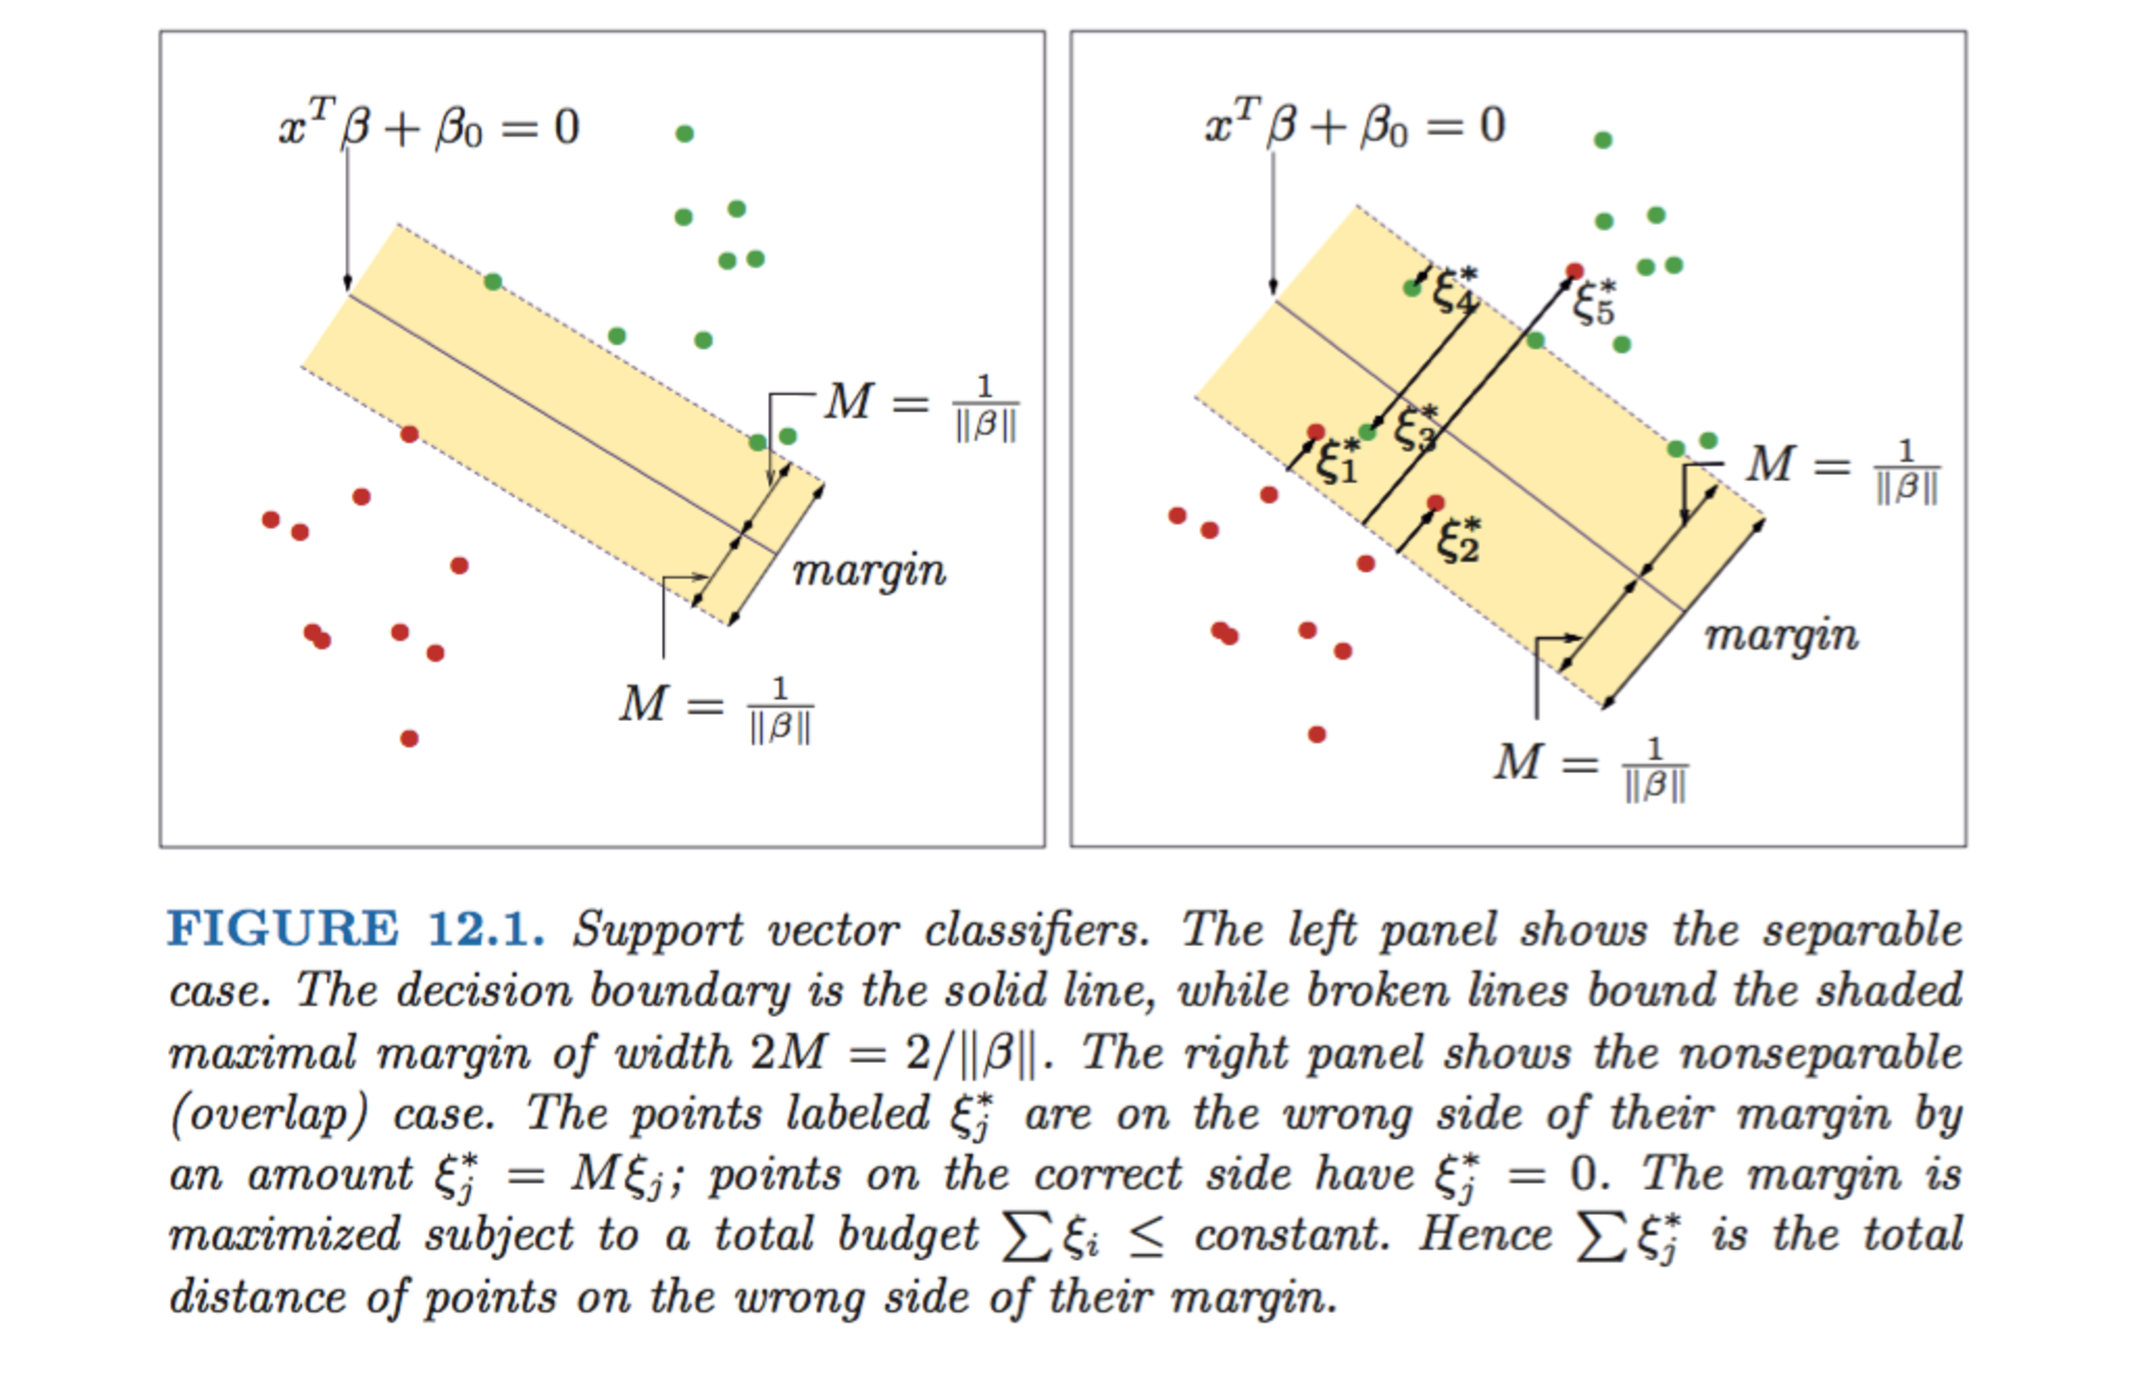
\includegraphics[height=0.7\textheight]{img/slack.pdf}
\end{center}

\end{frame}

%%%%%%%%%%%%%%%%%%%%%%%%%%%%%%%%%%%%%%%%%%%%%%%%%%%
\begin{frame}[fragile] \frametitle{} \oldB \small

Notice that we can rewrite
\begin{align*}
\min \quad &  \frac{1}{2} || \beta ||_2^2 \\
\text{s.t.} \quad & y_i (x_i^t \beta + \beta_0) > 1 - \xi_i, \quad i = 1, \ldots, n \\
&\xi_i > 0, \, \sum_i \xi_i \leq \text{Constant}
\end{align*}
With a constant $C > 0$, which depends only on the constant in the original
formulation, as:
\begin{align*}
\min \quad &  \frac{1}{2} || \beta ||_2^2 + \blue{C \cdot \sum_i \xi_i} \\
\text{s.t.} \quad & y_i (x_i^t \beta + \beta_0) > 1 - \xi_i, \quad \xi_i > 0, \quad i = 1, \ldots, n.
\end{align*}
By noticing that the second form will find a $\widehat{\beta}$ that minimizes
$|| \beta ||_2^2$ such that $\sum_i \xi_i \leq \sum_i \widehat{\xi}_i$.

\end{frame}

%%%%%%%%%%%%%%%%%%%%%%%%%%%%%%%%%%%%%%%%%%%%%%%%%%%
\begin{frame}[fragile] \frametitle{} \oldB \small

\textbf{The Lagrangian}

Given a constrained optimization problem:
\begin{align*}
\min &f(x) \\
\text{s.t.} \, &g_j(x) = 0, \quad \quad j = 1, \ldots, K
\end{align*}
We can define the primal Lagrangian function as:
\begin{align*}
\mathcal{L}_P &= f(x) - \sum_{j=1}^K \lambda_j g_j(x)
\end{align*}
What does this function look like?

\end{frame}

%%%%%%%%%%%%%%%%%%%%%%%%%%%%%%%%%%%%%%%%%%%%%%%%%%%
\begin{frame}[fragile] \frametitle{} \oldB \small

\textbf{The Lagrangian Dual}

The Lagrangian dual function is then given as the infimum
of $\mathcal{L}_P$ as function of the $\lambda_j$ over
values of $x$:
\begin{align*}
\mathcal{L}_D(\lambda) &= \inf_{x} \mathcal{L}_P(x,\lambda) \\
&=\inf_{x} \left\{ f(x) - \sum_{j=1}^K \lambda_j g_j(x)  \right\}.
\end{align*}
And the \textbf{dual problem} is to find the maximum of the
dual function over all choices of $\lambda$:
\begin{align*}
\lambda^{*} &= \argmax_{\lambda} \mathcal{L}_D(\lambda).
\end{align*}
The optimal value of the primal problem, $x^{*}$, can be reconstructed
by working backwards:
\begin{align*}
x^{*} &= \argmin_{x} \mathcal{L}_P(x, \lambda^{*}).
\end{align*}

\end{frame}

%%%%%%%%%%%%%%%%%%%%%%%%%%%%%%%%%%%%%%%%%%%%%%%%%%%
\begin{frame}[fragile] \frametitle{} \oldB \small

For a better understanding of the dual problem we can visualize the
Lagrangian solution as a saddle point\footnote{www.convexoptimization.com \\}

\vspace{-0in}

\begin{center}
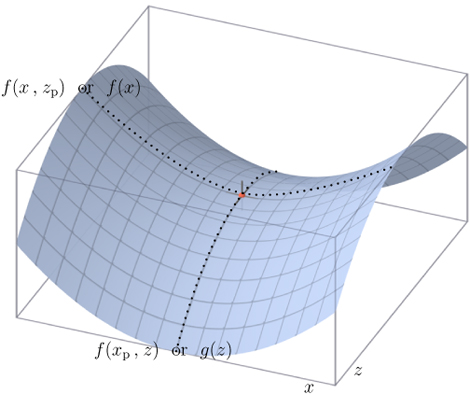
\includegraphics[height=2.5in]{img/saddle}
\end{center}

\end{frame}

%%%%%%%%%%%%%%%%%%%%%%%%%%%%%%%%%%%%%%%%%%%%%%%%%%%
\begin{frame}[fragile] \frametitle{} \oldB \small

It turns out that this is a very good framework for working with
support vector machines. We can define the Lagrangian function as:
\begin{align*}
\mathcal{L}_P &= \frac{1}{2} || \beta ||_2^2 + C \sum_i \xi_i
  - \sum_i \alpha_i \left[ y_i (x_i^t \beta + \beta_0) - (1 - \xi_i) \right]
  - \sum_i \mu_i \xi_i
\end{align*}
Where $\alpha_i$ and $\mu_i$ are the Lagrangian multipliers.

\end{frame}

%%%%%%%%%%%%%%%%%%%%%%%%%%%%%%%%%%%%%%%%%%%%%%%%%%%
\begin{frame}[fragile] \frametitle{} \oldB \small

\textbf{Aside:}

Technically, the theory of Lagrangian multipliers only apply when the
constraints on the solution are equality constraints rather than
inequality constraints. The larger theory needed for the general case
uses the \textit{Karush-Kuhn-Tucker} (KKT) conditions. These add
additional constraints on top of those presented here. Following
the Elements of Statistical Learning, we will not worry with those
details here as they are more an annoyance than an interesting
conceptual difference.

\end{frame}

%%%%%%%%%%%%%%%%%%%%%%%%%%%%%%%%%%%%%%%%%%%%%%%%%%%
\begin{frame}[fragile] \frametitle{} \oldB \small

To construct the dual function, we need to take partial derivatives with
respect to the primal variables: $\beta$, $\beta_0$, and $\xi_i$. If we
plug these into the primal problem, we get the dual function.

\end{frame}

%%%%%%%%%%%%%%%%%%%%%%%%%%%%%%%%%%%%%%%%%%%%%%%%%%%
\begin{frame}[fragile] \frametitle{} \oldB \small

For $\beta_j$:
\begin{align*}
\frac{\partial\mathcal{L}_P}{\partial \beta_j} &= \frac{\partial}{\partial \beta_j}
\left\{\frac{1}{2} || \beta ||_2^2 + C \cdot \sum_i \xi_i
  - \sum_i \alpha_i \left[ y_i (x_i^t \beta + \beta_0) - (1 - \xi_i) \right]
  - \sum_i \mu_i \xi_i \right\} \\
  &= \frac{\partial}{\partial \beta_j} \left\{\frac{1}{2} || \beta ||_2^2
  - \sum_i \alpha_i y_i (x_i^t \beta) \right\} \\
  &= \beta_j - \sum_i \alpha_i y_i x_{i,j}
\end{align*}
\pause Setting this equal to zero, and writing the equation simultaneously for all $\beta_j$,
we get:
\begin{align*}
\beta &= \sum_i \alpha_i y_i x_i
\end{align*}

\end{frame}

%%%%%%%%%%%%%%%%%%%%%%%%%%%%%%%%%%%%%%%%%%%%%%%%%%%
\begin{frame}[fragile] \frametitle{} \oldB \small

This necessary condition for the solution of the support vector machine is
of independent interest. It says that $\beta$ can be written as a linear
combination of the data points $x_i$. Any $i$ such that $\alpha_i$ is non-zero
is called a \magenta{support vector}.

\end{frame}

%%%%%%%%%%%%%%%%%%%%%%%%%%%%%%%%%%%%%%%%%%%%%%%%%%%
\begin{frame}[fragile] \frametitle{} \oldB \small

For $\beta_0$, the derivative is given as:
\begin{align*}
\frac{\partial\mathcal{L}_P}{\partial \beta_0} &= \frac{\partial}{\partial \beta_0}
\left\{\frac{1}{2} || \beta ||_2^2 + C \cdot \sum_i \xi_i
  - \sum_i \alpha_i \left[ y_i (x_i^t \beta + \beta_0) - (1 - \xi_i) \right]
  - \sum_i \mu_i \xi_i \right\} \\
  &= \frac{\partial}{\partial \beta_0}
    \left\{ - \sum_i \alpha_i y_i \beta_0 \right\} \\
  &= - \sum_i \alpha_i y_i
\end{align*}
Which when set to zero gives:
\begin{align*}
0 &= \sum_i \alpha_i y_i
\end{align*}
This explains why the term $\beta_0$ is often called the \magenta{bias} of
the support vector machine.

\end{frame}

%%%%%%%%%%%%%%%%%%%%%%%%%%%%%%%%%%%%%%%%%%%%%%%%%%%
\begin{frame}[fragile] \frametitle{} \oldB \small

Finally, the derivative with respect to $\xi_i$ is given as:
\begin{align*}
\frac{\partial\mathcal{L}_P}{\partial \xi_i} &= \frac{\partial}{\partial \xi_i}
\left\{\frac{1}{2} || \beta ||_2^2 + C \cdot \sum_i \xi_i
  - \sum_i \alpha_i \left[ y_i (x_i^t \beta + \beta_0) - (1 - \xi_i) \right]
  - \sum_i \mu_i \xi_i \right\} \\
  &= \frac{\partial}{\partial \xi_i}
    \left\{ C \cdot \sum_i \xi_i + \sum_i \alpha_i (1 - \xi_i) - \sum_i \mu_i  \right\} \\
  &= C - \alpha_i - \mu_i
\end{align*}
\pause Setting this equal to zero we see that:
\begin{align*}
\alpha_i &= C - \mu_i.
\end{align*}

\end{frame}

%%%%%%%%%%%%%%%%%%%%%%%%%%%%%%%%%%%%%%%%%%%%%%%%%%%
\begin{frame}[fragile] \frametitle{} \oldB \small

We now want to plug this into the Lagrangian primal function.
We first use the fact that $\alpha_i = C - \mu_i$ to unite the
trailing terms with respect to $\alpha_i$:
\begin{align*}
\mathcal{L}_D &= \frac{1}{2} || \beta ||_2^2 + \blue{C \sum_i \xi_i}
  - \sum_i \alpha_i \left[ y_i (x_i^t \beta + \beta_0) - (1 - \xi_i) \right]
  - \blue{\sum_i \mu_i \xi_i} \\
&= \frac{1}{2} || \beta ||_2^2 + \blue{\sum_i (C - \mu_i) \xi_i}
  - \sum_i \alpha_i y_i x_i^t \beta  - \sum_i \alpha_i y_i \beta_0 + \sum_i \alpha_i (1 - \xi_i) \\
&= \frac{1}{2} || \beta ||_2^2 + \blue{\sum_i \alpha_i \xi_i}
  - \sum_i \alpha_i y_i x_i^t \beta  - \sum_i \alpha_i y_i \beta_0 +
      \magenta{\sum_i \alpha_i (1 - \xi_i)}\\
&= \frac{1}{2} || \beta ||_2^2 + \magenta{\sum_i \alpha_i}
  - \sum_i \alpha_i y_i x_i^t \beta  - \sum_i \alpha_i y_i \beta_0
\end{align*}
\pause And the last term drops out:
\begin{align*}
\mathcal{L}_D &= \frac{1}{2} || \beta ||_2^2 + \sum_i \alpha_i
  - \sum_i \alpha_i y_i x_i^t \beta  - \magenta{\beta_0 \sum_i \alpha_i y_i} \\
  &= \frac{1}{2} || \beta ||_2^2 + \sum_i \alpha_i
  - \sum_i \alpha_i y_i x_i^t \beta
\end{align*}

\end{frame}

%%%%%%%%%%%%%%%%%%%%%%%%%%%%%%%%%%%%%%%%%%%%%%%%%%%
\begin{frame}[fragile] \frametitle{} \oldB \small

Now, notice that since $\beta = \sum_i \alpha_i y_i x_i$,
we have that:
\begin{align*}
|| \beta ||_2^2 &= \sum_j \beta_j^2 \\
&= \sum_{i'} \sum_i (\alpha_i y_i x_i)^t (\alpha_{i'} y_{i'} x_{i'}) \\
&= \sum_{i'} \sum_i \alpha_i \alpha_{i'} y_i y_{i'} x_i^t x_{i'}
\end{align*}
Also see that we can rewrite the last term in our dual function
as:
\begin{align*}
\sum_i \alpha_i y_i x_i^t \beta &= \sum_{i'} \sum_i \alpha_i \alpha_{i'} y_i y_{i'} x_i^t x_{i'} \\
&= || \beta ||_2^2.
\end{align*}

\end{frame}


%%%%%%%%%%%%%%%%%%%%%%%%%%%%%%%%%%%%%%%%%%%%%%%%%%%
\begin{frame}[fragile] \frametitle{} \oldB \small

Finally, the dual function can be written as:
\begin{align*}
\mathcal{L}_D &= \blue{\frac{1}{2} || \beta ||_2^2} + \sum_i \alpha_i
  - \blue{\sum_i \alpha_i y_i x_i^t \beta} \\
  &= \sum_i \alpha_i - \blue{\frac{1}{2} || \beta ||_2^2} \\
  &= \sum_i \alpha_i - \frac{1}{2} \cdot \blue{\sum_{i'} \sum_i \alpha_i \alpha_{i'} y_i y_{i'} x_i^t x_{i'}}.
\end{align*}
Which we want to maximize under the constraints (the first is
from the KKT conditions, the second from the partial derivative
of the bias):
\begin{align*}
0 \leq \alpha_i \leq C, \quad \sum_i \alpha_i y_i = 0.
\end{align*}

\end{frame}

%%%%%%%%%%%%%%%%%%%%%%%%%%%%%%%%%%%%%%%%%%%%%%%%%%%
\begin{frame}[fragile] \frametitle{} \oldB \small

To what extent can we make some sense of this equation?
First notice the duality of the problem if we flip the
$\pm 1$ labeling of the classes $y_i$:
\begin{align*}
\mathcal{L}_D &= \sum_i \alpha_i - \frac{1}{2} \cdot \sum_{i'} \sum_i \alpha_i \alpha_{i'} \blue{y_i y_{i'}}
x_i^t x_{i'}
\end{align*}
The function only depends on the sign of $y_i y_{i'}$. Also
note that it only depends on the data that serve as support
vectors:
\begin{align*}
\mathcal{L}_D &= \sum_i \blue{\alpha_i} - \frac{1}{2} \cdot \sum_{i'} \sum_i \blue{\alpha_i \alpha_{i'}} y_i y_{i'}
x_i^t x_{i'}.
\end{align*}

\end{frame}

%%%%%%%%%%%%%%%%%%%%%%%%%%%%%%%%%%%%%%%%%%%%%%%%%%%
\begin{frame}[fragile] \frametitle{} \oldB \small

Perhaps most importantly though, notice that only the
outer product $XX^t$ effects the final results:
\begin{align*}
\mathcal{L}_D &= \sum_i \alpha_i - \frac{1}{2} \cdot \sum_{i'} \sum_i \alpha_i \alpha_{i'} y_i y_{i'}
\blue{x_i^t x_{i'}}.
\end{align*}
As $x_i^t x_{i'}$ is the $(i,i')$'th element of $X X^t$. This is a measurement
of how similar $x_i$ and $x_{i'}$ are to one another (if scaled to both have
length one, it is the cosine of the angle between them).

\pause So, we can see that:
\begin{enumerate}
\item There is a penalty for including two similar $x_i$'s with the same class label
\item There is a benefit for including two similar $x_i$'s with different class labels
\end{enumerate}
Both of which actually make sense for a classification algorithm.

\end{frame}

%%%%%%%%%%%%%%%%%%%%%%%%%%%%%%%%%%%%%%%%%%%%%%%%%%%
\begin{frame}[fragile] \frametitle{} \oldB \small

Taking a step back now, how does logistic regression and support vector
machines compare?
\begin{enumerate}
\item Both separate the plane into two half-spaces which attempt to
split the classes as well as possible
\item However, logistic regression is (primarily) concerned with the
correlation matrix $X^t X$ between the variables and support vector machines
only care about the similarity matrix $X X^t$ between observations
\end{enumerate}

\end{frame}

%%%%%%%%%%%%%%%%%%%%%%%%%%%%%%%%%%%%%%%%%%%%%%%%%%%
\begin{frame}[fragile] \frametitle{} \oldB \small

\textbf{\yblue{The Kernel Trick}}

In the case of logistic and linear regression I have shown how basis
expansion can be used to add non-linear effects into a linear model.
One observation that makes support vector machines attractive is that
it is possible to mimic basis expansion without ever having to actually
project into a higher dimensional space.

\end{frame}

%%%%%%%%%%%%%%%%%%%%%%%%%%%%%%%%%%%%%%%%%%%%%%%%%%%
\begin{frame}[fragile] \frametitle{} \oldB \small

\textbf{\yblue{The Kernel Trick, cont.}}

Assume that we have a mapping $h$ of samples $x$ into a higher
dimensional space. We can re-write the dual function using
inner product notation:
\begin{align*}
\mathcal{L}_D &= \sum_i \alpha_i - \frac{1}{2} \cdot \sum_{i'} \sum_i \alpha_i \alpha_{i'} y_i y_{i'}
\blue{< h(x_i), h(x_{i'})>}.
\end{align*}
It quickly becomes apparent that we only need a fast way of
calculating inner products in the space of $h$, which may
not require actually determining and calculating $h$ itself.

\end{frame}

%%%%%%%%%%%%%%%%%%%%%%%%%%%%%%%%%%%%%%%%%%%%%%%%%%%
\begin{frame}[fragile] \frametitle{} \oldB \small

\textbf{\yblue{The Kernel Trick, cont.}}

The projected inner product $< h(x_i), h(x_{i'})>$ is usually
written directly as $K(x_i, x_{i'})$ for a function $K$ called
the kernel. Popular choices include:
\begin{enumerate}
\item \textbf{Linear:} $K(x, x') = <x, x'>$
\item \textbf{Polynomial:} $K(x, x') = (1 + <x, x'>)^d$
\item \textbf{Radial:}  $K(x, x') = exp(- \gamma || x - x' ||^2)$
\item \textbf{Sigmoid:}  $K(x, x') = tanh(\kappa_1 <x, x'> + \kappa_2)$
\end{enumerate}
Notice that these all require approximately the same effort to calculate as
the linear kernel.

\end{frame}

%%%%%%%%%%%%%%%%%%%%%%%%%%%%%%%%%%%%%%%%%%%%%%%%%%%
\begin{frame}[fragile] \frametitle{} \oldB \small

\textbf{\yblue{Finishing the optimization}}

Now, we can re-write the optimization problem as:
\begin{align*}
\max \quad& 1^t \alpha - \alpha^t K \alpha\\
\text{s.t.} \quad& 0 \leq \alpha_i \leq C
\end{align*}
For a suitable matrix $K$, called the kernel matrix.
This is a quadratic program with box constraints, and
can be solved fairly efficiently by general purpose
solvers.

\end{frame}

%%%%%%%%%%%%%%%%%%%%%%%%%%%%%%%%%%%%%%%%%%%%%%%%%%%
\begin{frame}[fragile] \frametitle{} \oldB \small

\textbf{\yblue{More information}}

I try to provide additional references for all of my lectures
on the class website. For today's material (and Wednesday's)
I would like to make a particular point to mention two references:
\begin{itemize}
\item Elements of Statistical Learning, Sections 12.1-12.4
\item Convex Optimization, S. Boyd, Chapter 5 (5.5 in particular)
\end{itemize}
These contain many more details than I have time to cover,
and assume a deeper background in statistics / convex calculus.

\end{frame}

\end{document}











